% \documentclass{article} 
\documentclass[12pt,english]{article}
% \pagestyle{headings}
% \usepackage[utf8]{inputenc}
% \usepackage{esvect}
% \usepackage{tikzpagenodes}
% \usepackage{tikz}
% \usepackage{graphicx}
% \usepackage[none]{hyphenat}
\usepackage{amsmath}
% \usepackage{stix}
% \usepackage{graphicx}
% \usepackage[square, numbers]{natbib}



\usepackage[T1]{fontenc}
\usepackage{babel}
\usepackage{graphicx}
\graphicspath{{../images/}}

\author{
    Meisel, Carlos \\
  \and
  Juarez, Albert\\
  \and
    Quintero, Osvaldo\\
}
\title{Task 4 - Compressor Map}

\begin{document}
  \maketitle

\section*{Overview}
This folder contains the code for designing a row of the Compressor map for the Axial Compressor. This task is full of tables, which will be broken down into detail down below.

\vspace*{3pt}

\verb|task4_main.py| is the main file which calls the other files and runs the code. Readers are to run this code to perfom the analysis.

\vspace*{3pt}

\verb|Table2.1.csv| contains the data from Table 2.1 in Dr. Cizmas' notes. This data is used to calculate the values for the compressor map. This table is read in by \verb|task4_main.py| and is used to calculate the values for the compressor map. Table 2.1 is shown below:


\begin{center}
    \begin{tabular}{ c c c c c c c c c c }
     $\bar{n}$ & 0.5 & 0.6 & 0.7 & 0.8 & 0.9 & 1.0 & 1.05 & 1.1 \\ 
        $\bar{\eta_{base}}$ & 0.9 & 0.924 & 0.955 & 0.97 & 1.0 & 1.0 & 0.98 & 0.975 \\
        $\bar{\dot{m_{base}}}$ & 0.37 & 0.47 & 0.58 & 0.714 & 0.86 & 1.0 & 1.02 & 1.04 \\
        $\bar{\pi_{base}}$ & 0.47 & 0.51 & 0.59 & 0.7 & 0.82 & 1.0 & 1.1 & 1.2 \\
    \end{tabular}
    \end{center}

\vspace*{3pt}

Where; 
\begin{center}
    $\bar{n}$ = $\frac{n}{n_{ref}}$ 

    \vspace*{3pt}

    $\bar{\eta_{base}}$ = $\frac{\eta_{base}}{\eta_{ref}}$
    
    \vspace*{3pt}
    
    $\bar{\dot{m_{base}}}$ = $\frac{\dot{m_{base}}}{\dot{m_{ref}}}$
    
    \vspace*{3pt}
    
    $\bar{\pi_{base}}$ = $\frac{\pi^* _{base}}{\pi^* _{ref}}$
\end{center}

\vspace*{3pt}

\verb|Table2.3.csv| contains the data from Table 2.3 in Dr. Cizmas' notes. This data is used to calculate the values for the compressor map. This table is read in by \verb|task4_main.py| and is used to calculate the values for the compressor map. Table 2.3 is shown below:

\begin{center}
    \begin{tabular}{ c c c c c c c }
     $\frac{\bar{C_{a}}}{\bar{C_{a_{base}}}}$ & 0.8 & 0.9 & 1.0 & 1.1 & 1.2 \\ 
        $\frac{\eta}{\eta_{base}}$ & 0.92 & 0.98 & 1 & 0.97 & 0.88 \\
        $\frac{w}{w_{base}}$ & 1.25 & 1.12 & 1 & 0.9 & 0.82 \\ 
    \end{tabular}
    \end{center}

\vspace*{3pt}
    
    Where;
\begin{center}
    $w = \frac{h^{*}_{1}}{\eta} (\pi^{* \frac{\gamma - 1}{\gamma}} - 1)$
    
    \vspace*{3pt}
    
    $h^{*}_{1} = \frac{w \eta}{\pi^{* \frac{\gamma - 1}{\gamma}} - 1}$
\end{center}

\vspace*{3pt}

Similarly we can say,

\begin{center}
    $h^{*}_{1} = \frac{w_{base} \eta_{base}}{(\pi^{* \frac{\gamma-1}{\gamma}})_{base} - 1}$

\end{center}

\vspace*{3pt}

Making use of these equations, we can write the following:

\begin{center}
    $\pi^{ * } = \left[ 1 + ((\pi^{ * \frac{\gamma - 1}{\gamma}})_{base} -1) \frac{w \eta}{w_{base} \eta_{base}} \right] ^{\frac{\gamma}{\gamma - 1}}$
\end{center}

\verb|steps.py| contains the 4 different steps that Dr. Cizmas has outlined in his notes. The steps are as follows:

\begin{enumerate}
    \item Calculate $\pi^{*} = \pi^{*} (\bar{n}, \frac{\bar{C_{a}}}{\bar{C_{a_{base}}}})$ and $\frac{\pi^{*}}{\pi^{*}_{base} = f (\bar{n}, \frac{\bar{C_{a}}}{\bar{C_{a_{base}}}})}$, where where $\bar{n} \in (0.5, 1.1)$ and $\frac{\bar{C_a}}{\bar{C_{a base}}} \in (0.8, 1.2)$ producing a table as shown in Table 2.4.1 and Table 2.4.2. (Tables are in \verb|Table_2_4_1.csv| and \verb|Table_2_4_2.csv| respectively)
    \begin{center}
        \begin{tabular}{ c c c c c c c c }
            $\frac{\bar{C_{a}}}{\bar{C_{a_{base}}}}$ & 0.8 & 0.9 & 1.0 & 1.1 & 1.2 & $\bar{n}$ \\
            $\pi^{*}$ & 4.64045 & 4.38299 & 3.93091 & 3.39379 & 2.83897 & 0.5 \\
            $\pi^{*}$ & 5.07483 & 4.78063 & 4.26545 & 3.65607 & 3.03024 & 0.6 \\
            $\pi^{*}$ & 5.95028 & 5.57996 & 4.93454 & 4.17687 & 3.40661 & 0.7 \\
            $\pi^{*}$ & 7.16637 & 6.68649 & 5.85454 & 4.88616 & 3.91291 & 0.8 \\
            $\pi^{*}$ & 8.50639 & 7.90169 & 6.85818 & 5.65264 & 4.45332 & 0.9 \\
            $\pi^{*}$ & 10.5374 & 9.73710 & 8.36364 & 6.79104 & 5.24562 & 1.0 \\
            $\pi^{*}$ & 11.6748 & 10.7622 & 9.19999 & 7.41866 & 5.67803 & 1.05 \\
            $\pi^{*}$ & 12.8177 & 11.7906 & 10.0363 & 8.04337 & 6.10576 & 1.1 \\
        \end{tabular}

        \vspace*{3pt}

        \begin{tabular}{c c c c c c c c }
            $\frac{\bar{C_{a}}}{\bar{C_{a_{base}}}}$ & 0.8 & 0.9 & 1.0 & 1.1 & 1.2 & $\bar{n}$ \\
            $\frac{\pi^{*}}{\pi^{*}_{base}}$ & 1.18050 & 1.11501 & 0.99999 & 0.86336 & 0.72222 & 0.5 \\
            $\frac{\pi^{*}}{\pi^{*}_{base}}$ & 1.18975 & 1.12078 & 0.99999 & 0.85713 & 0.71042 & 0.6 \\
            $\frac{\pi^{*}}{\pi^{*}_{base}}$ & 1.20584 & 1.13079 & 1.0 & 0.84646 & 0.69036 & 0.7 \\
            $\frac{\pi^{*}}{\pi^{*}_{base}}$ & 1.22407 & 1.14210 & 0.99999 & 0.83459 & 0.66835 & 0.8 \\
            $\frac{\pi^{*}}{\pi^{*}_{base}}$ & 1.24033 & 1.15215 & 0.99999 &  0.82422 & 0.64934 & 0.9 \\
            $\frac{\pi^{*}}{\pi^{*}_{base}}$ & 1.25991 & 1.16422 & 1.0 & 0.81197 & 0.62719 & 1.0 \\
            $\frac{\pi^{*}}{\pi^{*}_{base}}$ & 1.26899 & 1.16980 & 0.99999 & 0.80638 & 0.617177 & 1.05 \\
            $\frac{\pi^{*}}{\pi^{*}_{base}}$ & 1.27712 & 1.17479 & 0.99999 & 0.80142 & 0.608364 & 1.1 \\
        \end{tabular}
    \end{center}

    \item Calculate $\frac{\bar{\dot{m}}}{\bar{\dot{m_{base}}}} = f (\bar{n}, \frac{\bar{C_{a}}}{\bar{C_{a_{base}}}})$, by making use of:
    
    \begin{center}
        $\frac{\bar{\dot{m}}}{\bar{\dot{m_{base}}}} = \frac{\bar{C_{a}}}{\bar{C_{a_{base}}}} \left[ \frac{\bar{\pi^{*}}}{\bar{\pi^{*}_{base}}} \right] ^{\frac{1}{3}}$
    \end{center}

    Similar to step 1. Table 2.5 is produced. (Table is in \verb|Table_2_5_csv|)

    \begin{center}
        \begin{tabular}{ c c c c c c c c }
            $\frac{\bar{C_{a}}}{\bar{C_{a_{base}}}}$ & 0.8 & 0.9 & 1.0 & 1.1 & 1.2 & $\bar{n}$ \\
            $\frac{\bar{\dot{m}}}{\bar{\dot{m_{base}}}}$ & 0.84549 & 0.93326 & 1.0 & 1.04743 & 1.07664 & 0.5 \\
            $\frac{\bar{\dot{m}}}{\bar{\dot{m_{base}}}}$ & 0.84769 & 0.93487 & 0.99999 & 1.04490 & 1.07074 & 0.6 \\
            $\frac{\bar{\dot{m}}}{\bar{\dot{m_{base}}}}$ & 0.85150 & 0.93764 & 1.0 & 1.04054 & 1.06057 & 0.7 \\
            $\frac{\bar{\dot{m}}}{\bar{\dot{m_{base}}}}$ & 0.85577 & 0.94076 & 0.99999 & 1.03566 & 1.04918 & 0.8 \\
            $\frac{\bar{\dot{m}}}{\bar{\dot{m_{base}}}}$ & 0.85955 & 0.94351 & 1.0 & 1.03135 & 1.03914 & 0.9 \\
            $\frac{\bar{\dot{m}}}{\bar{\dot{m_{base}}}}$ & 0.86404 & 0.94679 & 1.0 & 1.02622 & 1.02718 & 1.0 \\
            $\frac{\bar{\dot{m}}}{\bar{\dot{m_{base}}}}$ & 0.86612 & 0.94830 & 0.99999 & 1.02386 & 1.02169 & 1.05 \\
            $\frac{\bar{\dot{m}}}{\bar{\dot{m_{base}}}}$ & 0.86796 & 0.94965 & 0.99999 & 1.02175 & 1.01680 & 1.1 \\
        \end{tabular}
    \end{center}

    \item Calculate $\bar{\pi} = \bar{\pi} (\bar{n}, \frac{\bar{C_{a}}}{\bar{C_{a_{base}}}})$ and $\bar{\dot{m}} = \bar{\dot{m}} (\bar{n}, \frac{\bar{C_{a}}}{\bar{C_{a_{base}}}})$, by making use of:
    \begin{center}
        $\bar{\pi} = \bar{\pi_{base}} \frac{\pi^{*}}{\pi^{*}_{base}}$
    \end{center}

    Where $\bar{pi_{base}}$ comes from \verb|Table2.1.csv| and $\frac{\pi^{*}}{\pi^{*}_{base}}$ comes from \verb|Table_2_4_2.csv|. Similarly,
    \begin{center}
        $\bar{\dot{m}} = \bar{\dot{m_{base}}} \frac{\bar{\dot{m}}}{\bar{\dot{m_{base}}}}$
    \end{center}

    Where $\bar{\dot{m_{base}}}$ comes from \verb|Table2.1.csv| and $\frac{\bar{\dot{m}}}{\bar{\dot{m_{base}}}}$ comes from \verb|Table_2_5.csv|. 

    \item Calculate $\eta = \eta (\bar{n}, \frac{\bar{C_{a}}}{\bar{C_{a_{base}}}})$ using tables \verb|Table2.1.csv|, \verb|Table2.3.csv|.
    
    \item Lastly we are to draw the Compressor map, with axes of $\dot{m} \frac{\sqrt{T^{*}_{1}}}{p^{*}_{1}}$, $\pi^{*}$ and $\eta$. We also provide a drawing of the surge line. The map is drawn:
    
    \begin{center}
        % include the image but fit it to the page
        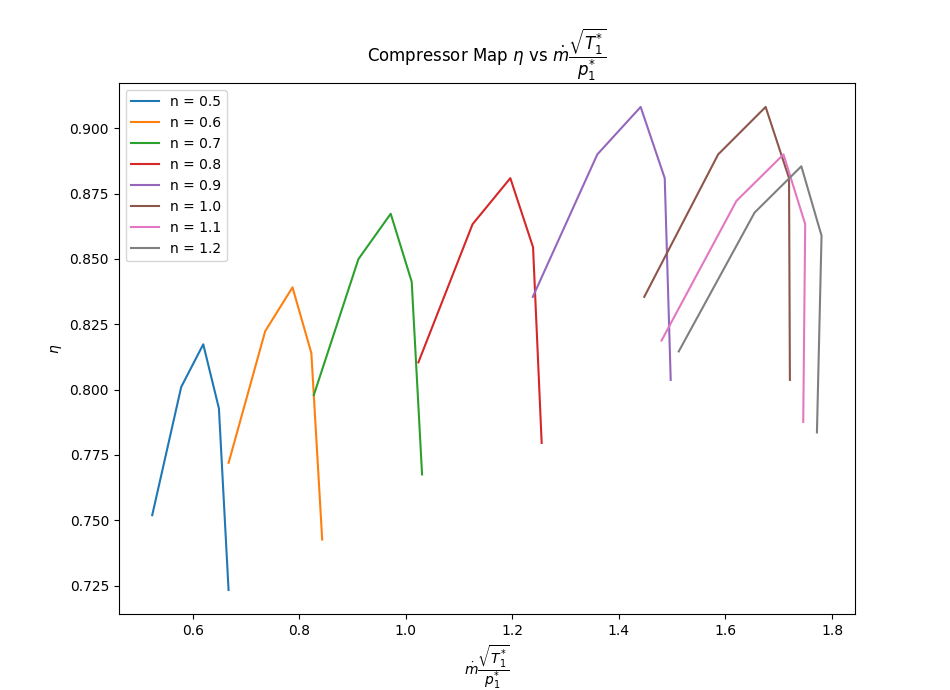
\includegraphics[width=\textwidth]{CompressorMap1.png}

    
        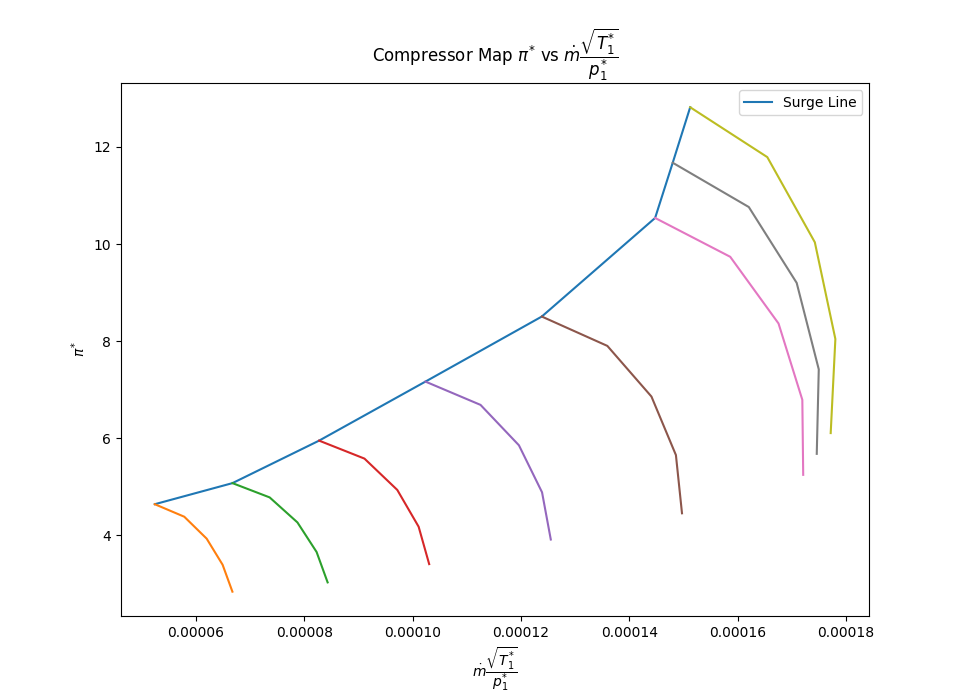
\includegraphics[width=\textwidth]{CompressorMap2.png}

        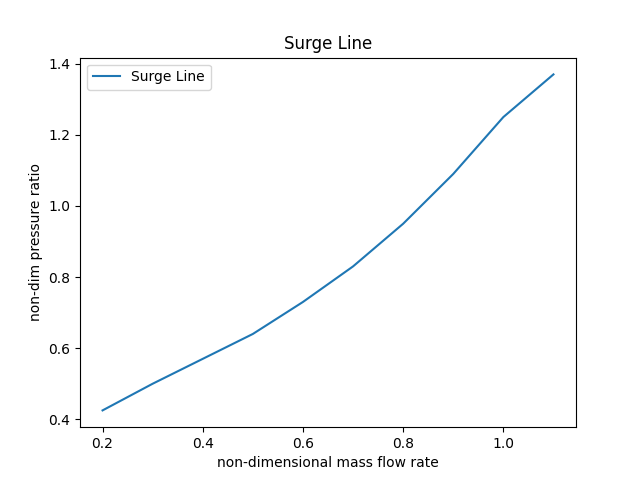
\includegraphics[width=\textwidth]{CompressorMap3.png}

    \end{center}
\end{enumerate}

\end{document}